\section{Implementação numérico-computacional e resultados}

Neste capítulo, será feita uma verificação numérico-computacional dos resultados analíticos obtidos nas seções anteriores empregando as técnicas do Funcional de Reciprocidade (FR) e da Transformada Integral Clássica (CITT) na estimativa da distribuição de condutância térmica de contato (CTC) ao longo de uma interface irregular segundo o arranjo proposto na figura \ref{fig2}. Este arranjo foi proposto como uma generalização da configuração estudada por \cite{tese_padilha}, na qual a interface de contato era uma superfície plana paralela às bases do corpo de prova.

Para tanto, diversos formatos de interface de contato foram propostos, bem como diferentes perfis de temperaturas medidas na superfície externa $\Gamma_0$ do corpo de prova. Para cada combinação composta por um formato de interface de contato e um perfil de temperaturas medidas na superfície externa, foi estimada, a partir das equações \eqref{calculo_FR_F1_antes}, \eqref{calculo_FR_G1_antes} e \eqref{expressao_final_ctc}, a distribuição da CTC na interface de contato referente a essa combinação, comparando-a com a distribuição de CTC teórica esperada para o caso. As medidas de temperatura na superfície externa correspondentes a uma determinada distribuição de CTC foram simuladas através da resolução do problema direto de condução de calor definido na seção \ref{sec_formulacao_direta} para a referida distribuição, e por isso são denominadas \textit{medidas sintéticas de temperatura}, ou simplesmente \textit{temperaturas sintéticas}.

Ainda seguindo a metodologia de trabalho conduzida por \cite{tese_padilha}, foram feitas simulações envolvendo erros experimentais nas medidas sintéticas de temperatura, e seus efeitos sobre a estimativa da distribuição da CTC.

\subsection{Configuração física e geométrica dos problemas-teste}\label{config_fis_geom}

Em todas as simulações, considerou-se que o corpo de prova representado na figura \ref{fig2} era composto de dois compósitos de materiais diferentes. Para o material superior $\Omega_1$ adotou-se o valor de condutividade térmica do aço AISI 1050, de 54 W/(m \celsius); para o material inferior $\Omega_2$, foi usado o valor de condutividade térmica do Incomel, de 14 W/(m \celsius). As dimensões do corpo de prova, ou seja, o comprimento e a altura da sua seção reta, foram respectivamente de 0,04 m e de 0,02 m. A superfície superior $\Gamma_0$ do corpo de prova foi submetida a um fluxo de calor por unidade de área de 100.000 W/$\text{m}^2$. Esses valores foram os mesmos adotados por \cite{tese_padilha} na condução do seu trabalho.

A Tabela \ref{tabela_params} sumariza os parâmetros físicos e geométricos usados no trabalho:
\vspace{10mm}
\begin{table}[H]
	\centering
	\caption{Parâmetros considerados nos problemas-teste}
	\begin{tabular}{@{}cc@{}}
		\toprule
		\textbf{Parâmetro} & \textbf{Valor}    \\ \midrule
		$a$       & 0,04 m   \\ \\
		$b$       & 0,02 m     \\ \\
		$k_1$     & 54 W/(m \celsius)  \\ \\ 
		$k_2$     & 14 W/(m \celsius) \\ \\
		$q$       & -100.000 W/$\text{m}^2$ \\ \bottomrule
	\end{tabular}		
\label{tabela_params}
\end{table}

Foram testadas três possibilidades de geometrias de interfaces de contato. Para cada uma delas foi associada uma equação da forma $y = w(x)$, descrevendo algebricamente a curva que representa cada interface. A Tabela \ref{tabela_interfaces} apresenta a definição das expressões de cada interface de contato.
\begin{table}[H]
	\centering
	\caption{Geometrias de interface de contato}
		\begin{tabular}{c|c}
			\hline \\
			\textbf{Geometria} & $w(x)$    \\ \\ \hline \\
			1       & $\displaystyle\frac{b}{2}$   \\ \\ \hline \\
			2       & $\begin{array}{ll}
			\displaystyle\frac{19bx^2}{8a^2}-\frac{7bx}{24a}+\frac{b}{2}, & \displaystyle 0 \le x < \frac{a}{3} \\ \\
			\displaystyle -\frac{25bx^2}{8a^2}+\frac{27bx}{8a}-\frac{b}{9}, & \displaystyle \frac{a}{3} \le x < \frac{2a}{3} \\ \\
			\displaystyle \frac{bx^2}{8a^2}-\frac{23bx}{24a}+\frac{4b}{3}, & \displaystyle \frac{2a}{3} \le x \le a
			\end{array}$     \\ \\ \hline \\
			3       & $\displaystyle \frac{b}{2} + \frac{1}{20} \cos\frac{4 \pi  x}{a}$ \\ \\ \hline
		\end{tabular}			
	\label{tabela_interfaces}
\end{table}

De forma a melhor ilustrar e visualizar as diferentes geometrias de interface de contato definidas acima, as suas representações gráficas são apresentadas na Figura \ref{figura_interfaces}.

\begin{figure}[h!b]
	\begin{minipage}[t][5cm][c]{\textwidth}
		\centering
		\begin{tikzpicture}
			\begin{axis}[
			anchor=east,  
			ticks=none,
			width=8cm,
			height=4cm,
			%ylabel=Iterações Lineares,
			xmin = 0,
			xmax = 0.04,
			ymin = 0,
			ymax = 0.02]
			\pgfplotstableread{../data/interface_01.dat} 
			\teff
			\addplot[color=blue,mark=none,smooth] table from \teff;
			\end{axis}
		\end{tikzpicture}
		\caption*{(a) Geometria 1}
	\end{minipage}
%	\begin{minipage}[t][5cm][t]{0,5\textwidth}
%		\begin{tikzpicture}
%		\begin{axis}[
%		anchor=east,  
%		ticks=none,
%		width=8cm,
%		height=4cm,
%		%ylabel=Iterações Lineares,
%		xmin = 0,
%		xmax = 0.04,
%		ymin = 0,
%		ymax = 0.02]
%		\pgfplotstableread{../data/interface_05.dat} 
%		\teff
%		\addplot[color=blue,mark=none,smooth] table from \teff;
%		\end{axis}
%		\end{tikzpicture}
%		\caption*{(b) Geometria 2}
%	\end{minipage}
%	\begin{minipage}[t][5cm][t]{0,5\textwidth}
%		\begin{tikzpicture}
%		\begin{axis}[
%		anchor=east,  
%		ticks=none,
%		width=8cm,
%		height=4cm,
%		%ylabel=Iterações Lineares,
%		xmin = 0,
%		xmax = 0.04,
%		ymin = 0,
%		ymax = 0.02]
%		\pgfplotstableread{../data/interface_06.dat} 
%		\teff
%		\addplot[color=blue,mark=none,smooth] table from \teff;
%		\end{axis}
%		\end{tikzpicture}
%		\caption*{(c) Geometria 3}
%	\end{minipage}
	\begin{minipage}[t][5cm][c]{\textwidth}
		\centering
		\begin{tikzpicture}
		\begin{axis}[
		anchor=east,  
		ticks=none,
		width=8cm,
		height=4cm,
		%ylabel=Iterações Lineares,
		xmin = 0,
		xmax = 0.04,
		ymin = 0,
		ymax = 0.02]
		\pgfplotstableread{../data/interface_02.dat} 
		\teff
		\addplot[color=blue,mark=none,smooth] table from \teff;
		\end{axis}
		\end{tikzpicture}
		\caption*{(d) Geometria 2}
	\end{minipage}
%	\begin{minipage}[t][5cm][t]{0,5\textwidth}
%		\begin{tikzpicture}
%		\begin{axis}[
%		anchor=east,  
%		ticks=none,
%		width=8cm,
%		height=4cm,
%		%ylabel=Iterações Lineares,
%		xmin = 0,
%		xmax = 0.04,
%		ymin = 0,
%		ymax = 0.02]
%		\pgfplotstableread{../data/interface_08.dat} 
%		\teff
%		\addplot[color=blue,mark=none,smooth] table from \teff;
%		\end{axis}
%		\end{tikzpicture}
%		\caption*{(e) Geometria 5}
%	\end{minipage}
	\begin{minipage}[t][5cm][c]{\textwidth}
		\centering
		\begin{tikzpicture}
		\begin{axis}[
		anchor=east,  
		ticks=none,
		width=8cm,
		height=4cm,
		%ylabel=Iterações Lineares,
		xmin = 0,
		xmax = 0.04,
		ymin = 0,
		ymax = 0.02]
		\pgfplotstableread{../data/interface_03.dat} 
		\teff
		\addplot[color=blue,mark=none,smooth] table from \teff;
		\end{axis}
		\end{tikzpicture}
		\caption*{(f) Geometria 3}
	\end{minipage}	
	\caption{Diferentes geometrias para a interface $\Gamma$}
	\label{figura_interfaces}
\end{figure}

\subsection{Perfis teóricos de condutância térmica de contato}\label{config_ctc}

Foram adotados três diferentes perfis de distribuição de CTC, extraídos do trabalho de \cite{tese_padilha} e trabalhos anteriores. Estes perfis estão listados na Tabela \ref{tabela_ctc}, onde $h_{max}$ corresponde ao valor máximo que a CTC pode assumir, fixado em 1000 W/($\text{m}^2$ \celsius), e $a$ é o comprimento do corpo de prova.
\begin{table}[H]
	\centering
	\caption{Perfis teóricos de condutância térmica de contato}
		\begin{tabular}{c|c}
			\hline \\
			\textbf{Perfil} & $h_c(x)$[W/($\text{m}^2$ \celsius)]  \\ \\ \hline \\
			\multirow{2}{*}{1} & $h_{max}$ para $x < a/4$ e $x > 3a/4$ \\ & 0 para $a/4 < x < 3a/4$ \\ \\ \hline \\
%			\multirow{2}{*}{2} & $h_{max}$ para $x < a/4$ e $a/2 < x < 3a/4$ \\ & 0 para $a/4 < x < a/2$ e $x > 3a/4$ \\ \\ \hline \\
			2 & $h_{max}\sin\displaystyle\frac{\pi x}{a}$ \\ \\ \hline \\
%			4 & $\abs{h_{max}\sin\displaystyle\frac{2\pi x}{a}}$ \\ \\ \hline \\
%			5 & $h_{max}$ \\ \\ \hline \\
			\multirow{3}{*}{3} & $h_{max}/2$ para $x < a/4$ e $a/2 < x < 3a/4$ \\ & $h_{max}$ para $a/4 < x < a/2$ \\ & 0 para $ x > 3a/4$
			\\ \\ \hline
		\end{tabular}			
	\label{tabela_ctc}
\end{table}

De forma a melhor ilustrar e visualizar os diferentes perfis definidos acima, as suas representações gráficas são apresentadas na Figura \ref{figura_ctc}.
\newpage
\begin{figure}[h!b]
	\begin{minipage}[t][5cm][c]{\textwidth}
		\centering		
		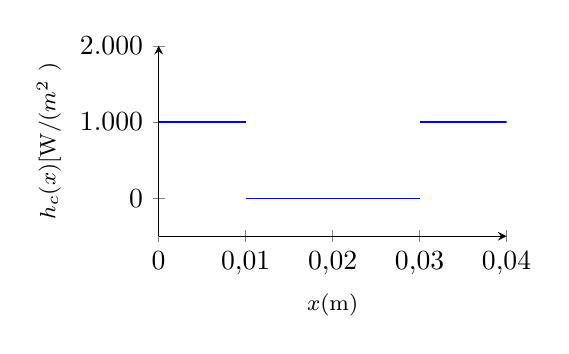
\begin{tikzpicture}
		\begin{axis}[
		/pgf/number format/1000 sep={.},/pgf/number format/use comma,
		axis lines=left,
		xmin = 0,
		xmax = 0.04,
		ymin = -500,
		ymax = 2000,
		restrict y to domain=-500:2000,
		scaled x ticks = false,
		scaled y ticks = false,
		x tick label style={/pgf/number format/fixed},
		y tick label style={/pgf/number format/fixed},
		anchor=east,  
		width=6cm,
		height=4cm,
		label style={font=\footnotesize},
		xlabel = $x$(m),
		ylabel= $h_c(x)[$W/($\text{m}^2$ \celsius)]]
		\addplot[color=blue,mark=none,smooth, domain=0:0.01] {1000};
		\addplot[color=blue,mark=none,smooth, domain=0.01:0.03] {0};
		\addplot[color=blue,mark=none,smooth, domain=0.03:0.04] {1000};
		\end{axis}
		\end{tikzpicture}
		\caption*{(a) Perfil 1}
	\end{minipage}
\end{figure}
%	\begin{minipage}[t][5cm][t]{0,5\textwidth}
%		\begin{tikzpicture}
%		\begin{axis}[
%		axis lines=left,
%		xmin = 0,
%		xmax = 0.04,
%		ymin = -500,
%		ymax = 2000,
%		restrict y to domain=-500:2000,
%		scaled x ticks = false,
%		scaled y ticks = false,
%		x tick label style={/pgf/number format/fixed},
%		y tick label style={/pgf/number format/fixed},
%		anchor=east,  
%		width=6cm,
%		height=4cm,
%		label style={font=\footnotesize},
%		xlabel = $x$(m),
%		ylabel= $h_c(x)$[W/($\text{m}^2$ \celsius)]]
%		\pgfplotstableread{../data/conductance_02.dat} 
%		\teff
%		\addplot[color=blue,mark=none,smooth] table from \teff;
%		\end{axis}
%		\end{tikzpicture}
%		\caption*{(a) Perfil 2}
%	\end{minipage}
\begin{figure}[h!b]
	\begin{minipage}[t][5cm][c]{\textwidth}
		\centering
		\begin{tikzpicture}
		\begin{axis}[
		/pgf/number format/1000 sep={.},/pgf/number format/use comma,
		axis lines=left,
		xmin = 0,
		xmax = 0.04,
		ymin = -500,
		ymax = 2000,
		restrict y to domain=-500:2000,
		scaled x ticks = false,
		scaled y ticks = false,
		x tick label style={/pgf/number format/fixed},
		y tick label style={/pgf/number format/fixed},
		anchor=east,  
		width=6cm,
		height=4cm,
		label style={font=\footnotesize},
		xlabel = $x$(m),
		ylabel= $h_c(x)$[W/($\text{m}^2$ \celsius)]]
		\pgfplotstableread{../data/conductance_02.dat} 
		\teff
		\addplot[color=blue,mark=none,smooth] table from \teff;
		\end{axis}
		\end{tikzpicture}
		\caption*{(a) Perfil 2}
	\end{minipage}
\end{figure}
\newpage
%	\begin{minipage}[t][5cm][t]{0,5\textwidth}
%		\begin{tikzpicture}
%		\begin{axis}[
%		axis lines=left,
%		xmin = 0,
%		xmax = 0.04,
%		ymin = -500,
%		ymax = 2000,
%		restrict y to domain=-500:2000,
%		scaled x ticks = false,
%		scaled y ticks = false,
%		x tick label style={/pgf/number format/fixed},
%		y tick label style={/pgf/number format/fixed},
%		anchor=east,  
%		width=6cm,
%		height=4cm,
%		label style={font=\footnotesize},
%		xlabel = $x$(m),
%		ylabel= $h_c(x)$[W/($\text{m}^2$ \celsius)]]
%		\pgfplotstableread{../data/conductance_04.dat} 
%		\teff
%		\addplot[color=blue,mark=none,smooth] table from \teff;
%		\end{axis}
%		\end{tikzpicture}
%		\caption*{(a) Perfil 4}
%	\end{minipage}
%	\begin{minipage}[t][5cm][t]{0,5\textwidth}
%		\begin{tikzpicture}
%		\begin{axis}[
%		axis lines=left,
%		xmin = 0,
%		xmax = 0.04,
%		ymin = -500,
%		ymax = 2000,
%		restrict y to domain=-500:2000,
%		scaled x ticks = false,
%		scaled y ticks = false,
%		x tick label style={/pgf/number format/fixed},
%		y tick label style={/pgf/number format/fixed},
%		anchor=east,  
%		width=6cm,
%		height=4cm,
%		label style={font=\footnotesize},
%		xlabel = $x$(m),
%		ylabel= $h_c(x)$[W/($\text{m}^2$ \celsius)]]
%		\pgfplotstableread{../data/conductance_05.dat} 
%		\teff
%		\addplot[color=blue,mark=none,smooth] table from \teff;
%		\end{axis}
%		\end{tikzpicture}
%		\caption*{(a) Perfil 5}
%	\end{minipage}
\begin{figure}[h!b]
	\begin{minipage}[t][5cm][c]{\textwidth}
		\centering
		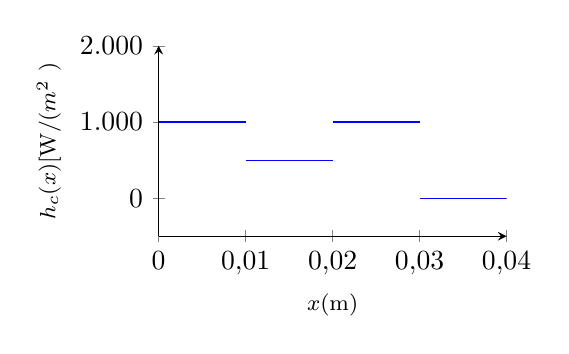
\begin{tikzpicture}
		\begin{axis}[
		/pgf/number format/1000 sep={.},/pgf/number format/use comma,
		axis lines=left,
		xmin = 0,
		xmax = 0.04,
		ymin = -500,
		ymax = 2000,
		restrict y to domain=-500:2000,
		scaled x ticks = false,
		scaled y ticks = false,
		x tick label style={/pgf/number format/fixed},
		y tick label style={/pgf/number format/fixed},
		anchor=east,  
		width=6cm,
		height=4cm,
		label style={font=\footnotesize},
		xlabel = $x$(m),
		ylabel= $h_c(x)$[W/($\text{m}^2$ \celsius)]]
		\addplot[color=blue,mark=none,smooth, domain=0:0.01] {1000};
		\addplot[color=blue,mark=none,smooth, domain=0.01:0.02] {500};
		\addplot[color=blue,mark=none,smooth, domain=0.02:0.03] {1000};
		\addplot[color=blue,mark=none,smooth, domain=0.03:0.04] {0};
		\end{axis}
		\end{tikzpicture}
		\caption*{(a) Perfil 3}
	\end{minipage}	
	\caption{Diferentes perfis de $h_c(x)$ na interface $\Gamma$}
	\label{figura_ctc}
\end{figure}


\subsection{Determinação das temperaturas sintéticas}

As medidas de temperatura na superfície superior $\Gamma_0$ do corpo de prova, representadas por $Y$ nas expressões \eqref{calculo_FR_F1_antes} e \eqref{calculo_FR_G1_antes}, foram obtidas resolvendo o problema direto definido na seção \ref{sec_formulacao_direta}, com os parâmetros, perfis de CTC e geometrias de interface indicados nas seções \ref{config_fis_geom} e \ref{config_ctc}. A fim de evitar a ocorrência do ``crime inverso", isto é, uma redução artificial do mal condicionamento do problema inverso quando o método empregado para resolvê-lo é o mesmo aplicado ao problema direto que fornece as medidas sintéticas\citep{livro_kaipio}, foram executadas simulações das diferentes configurações do problema direto no COMSOL \textit{Multiphysics}\textsuperscript{\textregistered}. O COMSOL é um \textit{software} comercial de elementos finitos, que possui um módulo específico para simulações de transferência de calor.

As várias configurações possíveis do problema direto definido na seção \ref{sec_formulacao_direta} foram modeladas e simuladas neste programa, seguindo os dados apresentados nas tabelas \ref{tabela_params}, \ref{tabela_interfaces} e \ref{tabela_ctc}, usando uma malha triangular extrafina. Para cada configuração, os valores de temperatura ao longo da interface superior $\Gamma_0$ foram exportados em arquivos-texto e usados como entrada para o programa implementado para a estimativa da CTC, e que será comentado na seção \ref{sobre_o_programa}. Convencionou-se extrair um total de 121 pontos equidistantes de medição de temperatura sobre a superfície $\Gamma_0$ para cada configuração.

Para fins de verificação, as mesmas combinações foram resolvidas numericamente através do método da Transformada Integral Clássica, e os resultados obtidos para a distribuição de temperaturas sobre a superfície $\Gamma_0$ apresentaram boa aderência com os obtidos a partir do COMSOL. A título de exemplo, as figuras \ref{fig_comparativo_1} e \ref{fig_comparativo_2} apresentam, respectivamente, um comparativo entre as temperaturas levantadas na superfície superior do corpo de prova, para a configuração específica referente à interface 3 e condutância de contato 1, e a distribuição do desvio relativo percentual entre essas medidas, calculada por:
\begin{align}
\epsilon_i = 100\abs{\frac{T\textsuperscript{COMSOL}_i - T\textsuperscript{CITT}_i}{T\textsuperscript{COMSOL}_i}}, i \in \Gamma_0
\end{align}

\begin{figure}[H]
	\begin{minipage}[t][8cm][c]{\textwidth}
		\centering
		\begin{tikzpicture}
		\begin{axis}[
		/pgf/number format/1000 sep={.},/pgf/number format/use comma,
		axis lines=left,
		%		xmin = 0,
		%		xmax = 0.04,
		%		ymin = 310,
		%		ymax = 340,
		%		restrict y to domain=-500:2000,
		scaled x ticks = false,
		scaled y ticks = false,
		x tick label style={/pgf/number format/fixed},
		y tick label style={/pgf/number format/fixed},
		anchor=east,  
		width=7cm,
		height=5cm,
		label style={font=\footnotesize},
		xlabel = $x$(m),
		ylabel= $T_1\big|_{\Gamma_0}$ (\celsius)]
		\pgfplotstableread{../data/fortran/temperaturas_sinteticas_interface_03_conductance_01.dat} 
		\teff
		\addplot[color=blue,mark=o,mark options={mark size=1.0pt}] table from \teff;
		\pgfplotstableread{../data/comsol/temperaturas_sinteticas_interface_03_conductance_01.dat} 
		\teff
		\addplot[only marks,color=red,mark=square,mark options={mark size=1.0pt}] table from \teff;
		\end{axis}
		\end{tikzpicture}
		\caption{Temperatura na superfície superior $\Gamma_0$ para a configuração referente à interface 3 e condutância de contato 1: $\textcolor{blue}{\ocircle} \rightarrow$ CITT; $\textcolor{red}{\square} \rightarrow$ Elementos finitos (COMSOL)}
		\label{fig_comparativo_1}
	\end{minipage}
	\begin{minipage}[t][8cm][c]{\textwidth}
		\centering
		\begin{tikzpicture}
		\begin{axis}[
		/pgf/number format/1000 sep={.},/pgf/number format/use comma,
		axis lines=left,
		%		xmin = 0,
		%		xmax = 0.04,
		%		ymin = 0.085,
		%		ymax = 0.105,
		%		restrict y to domain=-500:2000,
		scaled x ticks = false,
		scaled y ticks = false,
		x tick label style={/pgf/number format/fixed},
		y tick label style={/pgf/number format/fixed, /pgf/number format/precision=5},
		anchor=east,  
		width=7cm,
		height=5cm,
		label style={font=\footnotesize},
		xlabel = $x$(m),
		ylabel= $\epsilon$ (\%)]
		\pgfplotstableread{../data/desvio_relativo_interface_03_conductance_01.dat} 
		\teff
		\addplot[mark=o,mark options={mark size=1.0pt}] table from \teff;
		\end{axis}
		\end{tikzpicture}
		\caption{Desvio percentual entre as temperaturas obtidas via CITT e método dos elementos finitos (COMSOL), na superfície superior $\Gamma_0$ para a configuração referente à interface 3 e condutância de contato 1}
		\label{fig_comparativo_2}
	\end{minipage}
\end{figure}

As temperaturas sintéticas obtidas a partir do COMSOL correspondem a medidas consideradas exatas, sem ruídos ou erros experimentais. De forma a simular medidas com erros experimentais, foi implementado o mesmo procedimento adotado por \cite{tese_padilha}: foram adicionados erros randômicos com distribuição normal às temperaturas calculadas sobre a superfície superior do corpo de prova. Sendo então $\mathbf{Y}$ as medidas de temperatura simuladas sem erros, as medidas simuladas com erros, denotadas por $\tilde{\mathbf{Y}}$, foram calculadas através da expressão:
\begin{align}
\tilde{\mathbf{Y}} = \mathbf{Y} + \mathbf{\varepsilon} \sigma \label{modelagem_erro}
\end{align}
onde $\sigma$ é o desvio padrão das medidas de temperatura, e $\varepsilon$ é uma sequência aleatória gerada a partir da transformação Box-Muller\citep{artigo_box_muller}:
\begin{align}
\varepsilon = \cos(2\pi v)\sqrt{-2 \ln u}
\end{align}
onde $u$ e $v$ correspondem a variáveis aleatórias contínuas com distribuição uniforme entre 0 e 1.

Três níveis de desvio-padrão foram testados: $\sigma = \text{0,0}\celsius$ (correspondente aos casos onde as temperaturas sintéticas não contém erros), $\sigma = \text{0,1}\celsius$ e $\sigma = \text{0,5}\celsius$. Desse modo, havendo três possibilidades de geometrias de interface de contato e três possibilidades de condutância térmica de contato teórica, foram realizadas nove simulações distintas de problemas-teste diretos, para obtenção das respectivas distribuições de temperaturas sintéticas exatas. A cada um desses resultados foram aplicados os erros correpondentes às três possibilidades de desvio-padrão, num total de 27 conjuntos de dados de entrada; estes dados por sua vez alimentaram cada um dos 27 problemas inversos equivalentes resolvidos neste trabalho. Nas figuras \ref{figura_temperaturas_sinteticas_interface_01}, \ref{figura_temperaturas_sinteticas_interface_02} e \ref{figura_temperaturas_sinteticas_interface_03}, é possível visualizar as distribuições de temperaturas sintéticas na superfície superior do corpo de prova para cada uma das configurações. A maior ou menor dispersão dos dados com erros aleatórios em torno das medidas exatas é devida apenas às diferentes escalas adotadas no eixo $y$ de cada gráfico.

\begin{figure}[H]
	\graficostemperatura{1}{1}{a}{310}{345}
	\graficostemperatura{1}{2}{b}{251}{277}
	\graficostemperatura{1}{3}{c}{260}{330}
	\caption{Temperaturas sintéticas ($Y$) ao longo da superfície superior $\Gamma_0$, para os perfis de CTC de 1 a 3, referentes à interface de contato 1: $\textcolor{blue}{\ocircle} \rightarrow \sigma = 0,0$; $\textcolor{red}{\square} \rightarrow \sigma = 0,1$; $\textcolor{gray}{\triangle} \rightarrow \sigma = 0,5$}
	\label{figura_temperaturas_sinteticas_interface_01}
\end{figure}
\begin{figure}[H]
	\graficostemperatura{2}{1}{a}{310}{345}
	\graficostemperatura{2}{2}{b}{251}{277}
	\graficostemperatura{2}{3}{c}{260}{330}
	\caption{Temperaturas sintéticas ($Y$) ao longo da superfície superior $\Gamma_0$, para os perfis de CTC de 1 a 3, referentes à interface de contato 2: $\textcolor{blue}{\ocircle} \rightarrow \sigma = 0,0$; $\textcolor{red}{\square} \rightarrow \sigma = 0,1$; $\textcolor{gray}{\triangle} \rightarrow \sigma = 0,5$}
	\label{figura_temperaturas_sinteticas_interface_02}
\end{figure}
\begin{figure}[H]
	\graficostemperatura{3}{1}{a}{310}{345}
	\graficostemperatura{3}{2}{b}{251}{277}
	\graficostemperatura{3}{3}{c}{260}{330}
	\caption{Temperaturas sintéticas ($Y$) ao longo da superfície superior $\Gamma_0$, para os perfis de CTC de 1 a 3, referentes à interface de contato 3: $\textcolor{blue}{\ocircle} \rightarrow \sigma = 0,0$; $\textcolor{red}{\square} \rightarrow \sigma = 0,1$; $\textcolor{gray}{\triangle} \rightarrow \sigma = 0,5$}
	\label{figura_temperaturas_sinteticas_interface_03}
\end{figure}

\subsection{Interpolação das temperaturas sintéticas}\label{secao_interpolacao}
Sejam as expressões dos funcionais de reciprocidade associados às funções auxiliares $F_{1, j}$ e $G_{1, j}$, deduzidas no capítulo anterior:
\begin{align}
\Re(F_{1,j})
& =
-\frac{q}{k_1}\bar{\psi}_{j,0} + \frac{\mathbb{A}_{j,0} - \bar{\psi}_{j,0}}{ab}\int_0^a Y(x)dx + \nonumber \\
& \frac{2}{a}\sum_{m=1}^M \mu_m \left(\frac{\mathbb{A}_{j,m}}{\sinh\mu_m b} - \frac{\bar{\psi}_{j, m}}{\tanh\mu_m b}\right)\int_0^a Y(x)\cos\mu_m x dx
\label{calculo_FR_F1_antes_a} \\ \nonumber \\
\Re(G_{1,j})
& =
-\frac{q}{k_1}\bar{\phi}_{j,0} + \frac{\mathbb{E}_{j,0} - \bar{\phi}_{j,0}}{ab}\int_0^a Y(x)dx + \nonumber \\
& \frac{2}{a}\sum_{m=1}^M \mu_m \left(\frac{\mathbb{E}_{j,m}}{\sinh\mu_m b} - \frac{\bar{\phi}_{j, m}}{\tanh\mu_m b}\right)\int_0^a Y(x)\cos\mu_m x dx
\label{calculo_FR_G1_antes_a}
\end{align}

Foi comentado anteriormente que a função $Y(x)$ representa as medidas experimentais de temperatura na superfície superior do corpo de prova, obtidas artificialmente neste trabalho, através de simulação do problema direto. As integrais acima poderiam então ser imediatamente identificadas com a transformação integral da função $Y(x)$.

Na prática, porém, a função $Y(x)$ é desconhecida, e dispõe-se apenas de dados discretos, correspondentes às temperaturas medidas em pontos distintos da superfície superior. No trabalho de \cite{tese_padilha}, foi feita uma aproximação dessa função $Y(x)$ através de uma \textit{spline} que interpolava essas medidas. Uma outra forma de interpolar as medidas sintéticas, por meio de uma expansão em série de funções ortogonais às autofunções do problema de autovalor, foi proposta por \cite{artigo_mocerino} em seu trabalho de determinação de coeficiente de troca térmica de calor na parte interna de tubulações de trocadores de calor, que também empregou a técnica dos funcionais de reciprocidade. Desse modo, aplicando a segunda abordagem no caso em estudo, a função $Y(x)$ poderia ser escrita na forma
\begin{align}
Y(x) \approx \bar{y}_0 + \sum_{m=1}^M \bar{y}_m \cos\mu_m x \label{aproximacao_Y}
\end{align}

Não é difícil observar que a expressão acima é, basicamente, o truncamento da expansão de $Y(x)$ em somatório infinito de autofunções. Assim, podem-se estabelecer as seguintes relações entre os coeficientes $\bar{y}_m, m=0,1,2,...,M$ e as transformadas integrais de $Y(x)$:
\begin{align}
& \bar{y}_0 = \frac{1}{a}\int_0^a Y(x) dx \\ \nonumber \\
& \bar{y}_m = \frac{2}{a}\int_0^a Y(x) \cos\mu_m x dx, \qquad m = 1, 2, ..., M
\end{align}

Substituindo em \eqref{calculo_FR_F1_antes_a} e \eqref{calculo_FR_G1_antes_a}, obtém-se:
\begin{align}
\Re(F_{1,j})
& =
-\frac{q}{k_1}\bar{\psi}_{j,0} + \frac{\mathbb{A}_{j,0} - \bar{\psi}_{j,0}}{b} \bar{y}_0 + \sum_{m=1}^M \mu_m \left(\frac{\mathbb{A}_{j,m}}{\sinh\mu_m b} - \frac{\bar{\psi}_{j, m}}{\tanh\mu_m b}\right)\bar{y}_m
\label{calculo_FR_F1_antes_b} \\ \nonumber \\
\Re(G_{1,j})
& =
-\frac{q}{k_1}\bar{\phi}_{j,0} + \frac{\mathbb{E}_{j,0} - \bar{\phi}_{j,0}}{b} \bar{y}_0 + \sum_{m=1}^M \mu_m \left(\frac{\mathbb{E}_{j,m}}{\sinh\mu_m b} - \frac{\bar{\phi}_{j, m}}{\tanh\mu_m b}\right)\bar{y}_m
\label{calculo_FR_G1_antes_b}
\end{align}

Desse modo, as expressões \eqref{calculo_FR_F1_antes_b} e \eqref{calculo_FR_G1_antes_b} permitem determinar os funcionais de reciprocidade $\Re(F_{1,j})$ e $\Re(G_{1,j})$, apenas conhecendo os coeficientes $\bar{y}_0, \bar{y}_1, \bar{y}_2, ..., \bar{y}_M$ da aproximação \eqref{aproximacao_Y}. Estes coeficientes, por sua vez, podem ser calculados através da solução de aproximação por mínimos quadrados do problema, formulada a partir da aproximação sugerida em \eqref{aproximacao_Y}:
\begin{align}
\begin{bmatrix}
Y_0 \\ Y_1 \\ Y_2 \\ \vdots \\ Y_{imax}
\end{bmatrix}
=
\begin{bmatrix}
1 & \cos\mu_1 x_0 & \cos \mu_2 x_0 & ... & \cos\mu_M x_0 \\
1 & \cos\mu_1 x_1 & \cos \mu_2 x_1 & ... & \cos\mu_M x_1 \\
1 & \cos\mu_1 x_2 & \cos \mu_2 x_2 & ... & \cos\mu_M x_2 \\
... & ... & ... & \ddots & ... \\
1 & \cos\mu_1 x_{imax} & \cos \mu_2 x_{imax} & ... & \cos\mu_M x_{imax}
\end{bmatrix}
\times
\begin{bmatrix}
\bar{y}_0 \\ \bar{y}_1 \\ \bar{y}_2 \\ \vdots \\ \bar{y}_M
\end{bmatrix}
\label{sistema_aproximacao_Y}
\end{align}
onde cada par $(x_i, Y_i)$ corresponde respectivamente a um abscissa sobre a superfície superior do corpo de prova e o valor medido de temperatura naquele ponto.


\subsection{Definição das funções $\psi_j(x)$ e $\phi_j(x)$}
Uma questão que ficou em aberto até o momento é a que envolve a definição das funções $\psi_j(x)$ e $\phi_j(x)$, necessárias para a determinação das funções $\beta_j(x)$ e $\gamma_j(x)$. Neste trabalho foram empregadas as seguintes alternativas para estas funções:
\begin{align}
\psi_j(x), \phi_j(x) = \left\lbrace
\begin{array}{ll}
\displaystyle\sqrt{\frac{1}{a}}, & j = 0 \\ \nonumber \\
\displaystyle\sqrt{\frac{2}{a}}\cos \mu_j x, & j = 1,2,3,\ldots
\end{array}
\right.
\end{align} 

Estas funções foram as mesmas usadas por \cite{tese_padilha} na sua tese de doutorado e se mostraram bastante vantajosas do ponto de vista computacional, tanto neste como naquele trabalho. De fato, no estudo do problema de determinação da CTC numa interface plana horizontal no referido trabalho, foi demonstrado que o emprego destas funções diretamente nas condições de contorno dos problemas auxiliares para $F_{1,j}$, $F_{2,j}$ e $G_{1,j}$ garantia automaticamente a ortogonalidade das funções $\beta_j(x)$ e $\gamma_j(x)$. Já no presente trabalho, o grande benefício no uso destas funções reside na simplificação do cálculo das respectivas transformadas integrais:
\begin{align}
\bar{\psi}_{j, m}, \bar{\phi}_{j, m} = \left\lbrace
\begin{array}{ll}
\displaystyle\sqrt{\frac{a}{2}}, & j = m \ne 0 \\ \nonumber \\
\displaystyle\sqrt{a}, & j = m = 0 \\ \nonumber \\
0, & j \ne m 
\end{array}
\right.
\end{align}

\subsection{Código computacional}\label{sobre_o_programa}

Neste trabalho, o código computacional foi desenvolvido usando a linguagem de programação Fortran 2003. O compilador usado foi o \textit{gfortran}, que faz parte do projeto de \textit{software} livre GCC. O ambiente de desenvolvimento, onde o código era editado, compilado e depurado, foi o Eclipse, que também é um \textit{software} não-comercial. Todo o trabalho foi desenvolvido num computador executando o sistema operacional Linux para plataforma de 64 bits; no caso, a distribuição do sistema operacional usada foi Ubuntu versão 16.04.

As rotinas numéricas empregadas foram obtidas do projeto Netlib\footnote{Mais informações sobre o repositório Netlib podem ser encontradas no endereço de Internet \href{https://www.netlib.org/}{https://www.netlib.org/}.}, que é um repositório \textit{online} mantido por algumas instituições e universidades, contendo \textit{software} de computação científica e documentação disponíveis gratuitamente. A maioria das rotinas encontradas no repositório Netlib está escrita em FORTRAN 77\footnote{O uso de caixa alta para designar a versão 77 da linguagem Fortran tem raízes históricas, sendo encontrado em muitas publicações, e por isso esta convenção foi mantida aqui.}, especialmente as usadas no programa desenvolvido para este trabalho, o que não trouxe dificuldades, pois o compilador \textit{gfortran} é capaz de efetuar a compilação híbrida de arquivos-fonte escritos tanto em FORTRAN 77 quanto em Fortran 2003, inclusive padronizando para que todas as variáveis de ponto flutuante de precisão simples sejam tratadas como sendo de precisão dupla, o que de fato foi feito no programa.
A livre disponibilidade do código-fonte das rotinas facilitou significativamente a depuração do programa e a consequente identificação e correção de erros, sendo um fator determinante no desenvolvimento do mesmo. 

Foram empregadas rotinas numéricas do repositório Netlib para realizar as seguintes tarefas:
\begin{itemize}
	\item Cálculo dos coeficientes $\bar{y}_0, \bar{y}_1, \bar{y}_2, ..., \bar{y}_M$ presentes nas equações \eqref{calculo_FR_F1_antes_b} e \eqref{calculo_FR_G1_antes_b}, calculados a partir da solução de mínimos quadrados do sistema \eqref{sistema_aproximacao_Y}. O repositório Netlib possui o subprojeto LAPACK (\textit{Linear Algebra PACKage}), contendo diversos \textit{solvers} de sistemas lineares para várias possibilidades de matrizes de coeficientes: matrizes-banda, simétricas, positivas definidas, etc, além de outros utilitários de Álgebra Linear. Foi utilizada a rotina DGELS, que recebe a matriz e o vetor correspondentes ao sistema, e retorna a solução de mínimos quadrados, além de outras informações, tais como a norma dos resíduos.
%	\item Cálculo das integrais presentes nas equações \eqref{calculo_FR_F1_antes} e \eqref{calculo_FR_G1_antes}. Estas integrais são da forma
%	\begin{align}
%	& \int_0^a Y(x)dx \\ \nonumber \\
%	& \int_0^a Y(x)\cos\mu_m x dx
%	\end{align}
%	Estas integrais devem ser resolvidas numericamente, uma vez que o termo $Y(x)$, referente às temperaturas sintéticas sobre a superfície superior do corpo de prova, corresponde na verdade a um conjunto de dados discretos cuja formulação analítica é desconhecida (num problema real). Foram utilizadas duas rotinas que trabalhavam em conjunto: CURFIT, que aproxima um conjunto de pontos $(x_i, y_i)$ em uma B-\textit{spline}, e SPLINT, que integra a B-\textit{spline} obtida da rotina anterior sobre um intervalo.
	
	\item Cálculo das transformadas integrais que fornecem os coeficientes dos sistemas lineares \eqref{sistema_para_coeficientes_3} e \eqref{sistema_para_coeficientes_21}. O repositório Netlib oferece a rotina DQAWO, que faz parte do subprojeto QUADPACK, e que resolve integrais da forma
	\begin{align}
	& \int_{x_0}^{x_1} f(x)\cos\omega x dx \label{dqawo} \\ \nonumber \\
	& \int_{x_0}^{x_1} f(x)\sin\omega x dx 
	\end{align}
	A rotina foi parametrizada para resolver integrais conforme a expressão \eqref{dqawo}, fazendo $\omega = \mu_m$.
	
	\item Solução numérica dos sistemas de equações lineares \eqref{sistema_para_coeficientes_3} e \eqref{sistema_para_coeficientes_21}. Foi utilizada no trabalho a rotina DGESVX, do subprojeto LAPACK, que recebe como entrada a matriz de coeficientes e uma matriz cujas colunas são diferentes vetores de termos independentes do sistema; a rotina aplica um pré-condicionador ao sistema, realiza uma decomposição LU da matriz de coeficientes e usa este resultado para obter os vetores-solução referentes a cada vetor de termos independentes. Esta rotina atendeu à necessidade de se resolver de forma eficiente um dado sistema de equações, variando apenas o segundo membro correspondente aos termos independentes, o que foi comentado na seção \ref{orto_beta_gama}.
	
	\item Cálculo das integrais necessárias para a ortogonalização de Gram-Schmidt. Estas integrais, definidas de forma geral pela equação \eqref{integral_da_definicao_produto_interno_4}, foram calculadas através da rotina de integração de propósito geral DAQG, que realiza uma integração adaptativa através das fórmulas de quadratura de Gauss-Konrod.
\end{itemize}

Diversas otimizações foram implementadas a fim de minimizar o tempo de processamento, como por exemplo operações diretas com segmentos de matrizes e vetores ao invés de laços iterativos. Tais otimizações levaram a uma melhoria considerável no desempenho do programa como um todo, em especial na fase de ortonormalização de Gram-Schmidt, onde se observava o maior gargalo de processamento. Desse modo, o tempo de execução do código computacional no cálculo de um determinado perfil de condutância térmica de contato não excedia o intervalo de tempo de 2,5 segundos\footnote{Nas execuções realizadas num computador Lenovo Ideapad 330, com processador Intel Core\textsuperscript{\texttrademark} i5-8250U, CPU 1,60 GHz e memória RAM de 8 GB, o tempo total para o levantamento de uma estimativa de perfil de condutância térmica de contato variava entre 2,0 segundos a 2,4 segundos.}.

\subsection{Resultados e análises}

Serão apresentados agora os resultados numéricos obtidos a partir da aplicação das equações \eqref{calculo_FR_F1_antes}, \eqref{calculo_FR_G1_antes} e \eqref{expressao_final_ctc} ao problema inverso de condução de calor descrito no capítulo \ref{sec_prob_inv}. Estas equações fornecem, respectivamente, as estimativas de salto de temperatura, fluxo de calor e condutância térmica de contato na interface entre os materiais que compõem o arranjo físico ilustrado na figura \ref{fig2}.

Para cada combinação possível de geometria de interface (Tabela \ref{tabela_interfaces}), perfil de condutância térmica de contato (Tabela \ref{tabela_ctc}) e desvio-padrão de erros de medição ($\sigma = \text{0,0}\celsius$, $\sigma = \text{0,1}\celsius$ e $\sigma = \text{0,5}\celsius$), foram calculadas estimativas de salto de temperatura e fluxo de calor na interface de contato, e os resultados foram comparados com os respectivos valores teóricos esperados para cada combinação. A estimativa do perfil de condutância térmica de contato, calculada através da razão entre o fluxo de calor e o salto de temperatura estimados na interface, também foi comparada com o perfil teórico correspondente, e que foi usado para determinação prévia das temperaturas sintéticas através de simulações de cada configuração do problema no módulo de transferência de calor no simulador COMSOL \textit{Multiphysics}\textsuperscript{\textregistered}.

Não foi realizada uma análise de convergência rigorosa dos somatórios nas expressões \eqref{serie_para_beta}, \eqref{serie_para_gamma}, \eqref{calculo_FR_F1_antes_b} e \eqref{calculo_FR_G1_antes_b}, que fornecem as funções $\beta_j$ e $\gamma_j$ e os funcionais de reciprocidade, nem das equações \eqref{resultado_1} e \eqref{resultado_2}, que representam o fluxo de calor e o salto de temperatura na interface de contato. Adotou-se $M=20$ para o número de autofunções empregados nos somatórios que fornecem $\beta_j$, $\gamma_j$ e para o número de termos a serem somados para determinação de $\Re(F_{1,j})$ e $\Re(G_{1,j})$. Para o cálculo do salto de temperatura e do fluxo de calor na interface de contato, em todos os casos estudados foram assumidos os seguintes limites máximos para os índices dos somatórios correspondentes:
\begin{itemize}
	\item $N_1 \le 20$ (número máximo de funcionais de reciprocidade calculados para as expansões de salto de temperatura)
	\item $N_2 \le 20$ (número máximo de funcionais de reciprocidade calculados para as expansões de fluxo de calor)
\end{itemize}

Estes limites de somatórios permitiram a obtenção de resultados sem problemas de divergência ou estabilidade. Posteriormente serão tecidos comentários quanto ao caráter instável dos somatórios referentes aos cálculos do salto de temperatura e do fluxo de calor, bem quanto às dificuldades de estabelecimento de critérios de parada destes somatórios.

Os gráficos utilizados na análise estão agrupados por geometria de interface; em cada grupo, estão plotadas as estimativas de salto de temperatura e fluxo de calor na interface de contato. A estimativa da condutância térmica de contato é representada no último subgrupo de gráficos para cada interface.


\subsubsection{Estimativas para a geometria de interface de contato 1}

A primeira geometria de interface de contato para a qual foram realizadas estimativas de condutância térmica de contato é a referente ao índice 1 na tabela \ref{tabela_interfaces}. Esse formato de interface, basicamente uma superfície plana e horizontal paralela às bases do corpo de prova de seção reta retangular (cf. Figura \ref{figura_interfaces}), corresponde exatamente à configuração inicialmente estudada por \cite{reciproc_3}, e que culminou no trabalho desenvolvido por \cite{tese_padilha}. Esta configuração foi o ponto de partida das primeiras pesquisas envolvendo a aplicação do método dos Funcionais de Reciprocidade na estimativa da condutância térmica de contato. Desse modo, este problema-teste serviu como base de referência para verificação da metodologia proposta neste trabalho.

As estimativas para o salto de temperatura ao longo da interface de contato, correspondentes aos três perfis teóricos de CTC, estão plotadas nos gráficos da Figura \ref{figura_delta_temperaturas_interface_01}. Verificou-se uma excelente concordância entre as estimativas e os valores exatos; para o caso específico em que o desvio padrão é zero, as estimativas praticamente coincidiram com as medidas sintéticas. Notou-se também que as regiões em que o salto de temperatura atinge valores maiores correspondem às regiões onde a condutância térmica é menor. Assim, o comportamento da distribuição estimada do salto de temperatura mostrou-se consistente com o comportamento teórico esperado.
\begin{figure}[H]
	\graficoestimativa{delta_temperatura}{1}{1}{20}{06}{02}{a}{\Delta T\big|_{\Gamma}}{\celsius}
	\graficoestimativa{delta_temperatura}{1}{2}{20}{04}{04}{a}{\Delta T\big|_{\Gamma}}{\celsius}
	\graficoestimativa{delta_temperatura}{1}{3}{20}{06}{03}{a}{\Delta T\big|_{\Gamma}}{\celsius}
	\caption{Comparação entre as estimativas de $[T_1 - T_2]_\Gamma$ e os valores exatos para os perfis de CTC de 1 a 3, referentes à interface de contato 1: $\text{--} \rightarrow \text{Exato}$; $\textcolor{blue}{\ocircle} \rightarrow \sigma = 0,0$; $\textcolor{red}{\square} \rightarrow \sigma = 0,1$; $\textcolor{gray}{\triangle} \rightarrow \sigma = 0,5$}
	\label{figura_delta_temperaturas_interface_01}
\end{figure}

As estimativas para o fluxo de calor ao longo da interface de contato, correspondentes aos três perfis teóricos de CTC, estão plotadas nos gráficos da Figura \ref{figura_fluxo_calor_interface_01}. Novamente pôde ser observada uma boa coerência entre as estimativas e os valores exatos. No caso $\sigma = \text{0,0}\celsius$ em especial, nota-se a manifestação de um fenômeno semelhante ao efeito Gibbs\citep{livro_boyce} para os perfis de condutância teóricos 1 e 3, que apresentam descontinuidades. O comportamento qualitativo do fluxo de calor também foi consistente com o esperado; de fato, fluxos de calor mais altos correspondiam a regiões em que a condutância térmica era maior.
 
\begin{figure}[H]
	\graficoestimativa{fluxo_calor}{1}{1}{20}{06}{04}{a}{-k_1 \frac{\partial T_1}{\partial\mathbf{n}_1}\big|_{\Gamma}}{W/$\text{m}^2$}
	\graficoestimativa{fluxo_calor}{1}{2}{20}{04}{04}{a}{-k_1 \frac{\partial T_1}{\partial\mathbf{n}_1}\big|_{\Gamma}}{W/$\text{m}^2$}
	\graficoestimativa{fluxo_calor}{1}{3}{20}{06}{04}{a}{-k_1 \frac{\partial T_1}{\partial\mathbf{n}_1}\big|_{\Gamma}}{W/$\text{m}^2$}
	\caption{Comparação entre as estimativas de $[-k_1 {\partial T_1}/{\partial\mathbf{n}_1}]_\Gamma$ e os valores exatos para os perfis de CTC de 1 a 3, referentes à interface de contato 1: $\text{--} \rightarrow \text{Exato}$; $\textcolor{blue}{\ocircle} \rightarrow \sigma = 0,0$; $\textcolor{red}{\square} \rightarrow \sigma = 0,1$; $\textcolor{gray}{\triangle} \rightarrow \sigma = 0,5$}
	\label{figura_fluxo_calor_interface_01}
\end{figure}

Uma vez conhecidas as estimativas de fluxo de calor e salto de temperatura na interface de contato, a razão entre essas grandezas em cada ponto $x$ do domínio da interface ($0 \le x \le a$, onde $a$ é o comprimento do corpo de prova) fornece a estimativa do perfil de condutância térmica de contato, conforme a definição apresentada na equação \eqref{eq:definicao_3}. Desse modo, chega-se aos resultados representados graficamente na Figura \ref{figura_ctc_interface_01}\footnote{Os valores negativos de condutância térmica de contato, correspondentes aos perfis 1 e 3, não possuem significado físico, sendo consequência do comportamento oscilatório das funções $\psi_j(x)$ e $\phi_j(x)$ e das descontinuidades nestes perfis.}.
\begin{figure}[H]
	\graficoctc{01}{01}{1}{a}
	\graficoctc{01}{02}{2}{b}
	\graficoctc{01}{03}{3}{c}
	\caption{Comparação entre as estimativas de $h_c$ e os valores exatos para os perfis de CTC de 1 a 3, referentes à interface de contato 1: $\text{--} \rightarrow \text{Exato}$; $\textcolor{blue}{\ocircle} \rightarrow \sigma = 0,0$; $\textcolor{red}{\square} \rightarrow \sigma = 0,1$; $\textcolor{gray}{\triangle} \rightarrow \sigma = 0,5$}
	\label{figura_ctc_interface_01}
\end{figure}

Os gráficos acima apresentam excelente nível de aderência às soluções encontradas por \cite{tese_padilha} no seu trabalho, que contemplava a mesma interface de contato plana horizontal analisada nesta subseção. É interessante destacar este fato, pois a concordância com resultados obtidos em trabalhos anteriores é uma forma de verificação da corretude do desenvolvimento analítico conduzido neste trabalho.

Pode-se inferir, por observação dos gráficos \ref{figura_delta_temperaturas_interface_01}, \ref{figura_fluxo_calor_interface_01} e \ref{figura_ctc_interface_01}, que há uma relação direta e qualitativa entre a qualidade das previsões e o nível de ruído das medições de temperaturas na superfície superior do corpo de prova. De fato, esse é um resultado intuitivamente esperado: quanto menor for o desvio-padrão das medidas de temperatura, mais próxima será a estimativa em relação ao perfil teórico.

\subsubsection{Estimativas para a geometria de interface de contato 2}

A próxima geometria de interface de contato a ser analisada corresponde à de índice 2 na tabela \ref{tabela_interfaces}. Trata-se de uma curva polinomial definida por partes, ao longo do domínio $0 \le x \le a$, construída algebricamente de forma a garantir continuidade tanto na curva quanto na sua primeira derivada (cf. Figura \ref{figura_interfaces}). Os perfis estimados de salto de temperatura na interface de contato, correspondentes aos três perfis teóricos de CTC, podem ser visualizados na Figura \ref{figura_delta_temperaturas_interface_02}.
\begin{figure}[H]
	\graficoestimativa{delta_temperatura}{2}{1}{20}{11}{09}{a}{\Delta T\big|_{\Gamma}}{\celsius}
	\graficoestimativa{delta_temperatura}{2}{2}{20}{09}{07}{a}{\Delta T\big|_{\Gamma}}{\celsius}
	\graficoestimativa{delta_temperatura}{2}{3}{20}{11}{09}{a}{\Delta T\big|_{\Gamma}}{\celsius}
	\caption{Comparação entre as estimativas de $[T_1 - T_2]_\Gamma$ e os valores exatos para os perfis de CTC de 1 a 3, referentes à interface de contato 2: $\text{--} \rightarrow \text{Exato}$; $\textcolor{blue}{\ocircle} \rightarrow \sigma = 0,0$; $\textcolor{red}{\square} \rightarrow \sigma = 0,1$; $\textcolor{gray}{\triangle} \rightarrow \sigma = 0,5$}
	\label{figura_delta_temperaturas_interface_02}
\end{figure}

Novamente é possível observar uma boa aderência aos perfis teóricos calculados via simulação do problema direto correspondente. Os perfis estimados para $\sigma = 0,0\celsius$ são os que melhor se aproximam dos perfis esperados, ainda que apresentem alguma dificuldade de convergência nas extremidades do domínio.

Os gráficos da Figura \ref{figura_fluxo_calor_interface_02} mostram as estimativas para o fluxo de calor ao longo da interface de contato, correspondentes aos três perfis teóricos de CTC. Novamente a solução para $\sigma = 0,0\celsius$ é a que apresenta melhor concordância com o comportamento teórico esperado, muito embora as soluções encontradas para os outros valores de desvio-padrão também sejam muito boas, e possuam características qualitativas compatíveis com o esperado. O efeito Gibbs também pode ser observado nas estimativas de fluxo de calor referentes aos perfis teóricos descontínuos de CTC.

%
%\begin{figure}[h!b]
%	\graficoerrorms{norma}{delta_temperatura}{2}{1}{[T_1 - T_2]_\Gamma}{a}
%	\graficoerrorms{norma}{delta_temperatura}{2}{2}{[T_1 - T_2]_\Gamma}{b}
%	\graficoerrorms{norma}{delta_temperatura}{2}{3}{[T_1 - T_2]_\Gamma}{c}
%	\caption{Erro $\log[\text{RMS}(\delta)]$ das estimativas de $[T_1 - T_2]_\Gamma$ versus o número de funções ortonormais ($N_j$), para o perfis de CTC de 1 a 3, referentes à interface de contato 2: $\textcolor{blue}{\ocircle} \rightarrow \sigma = 0,0$; $\textcolor{red}{\square} \rightarrow \sigma = 0,1$; $\textcolor{gray}{\triangle} \rightarrow \sigma = 0,5$}
%\end{figure}
%
\begin{figure}[H]
	\graficoestimativa{fluxo_calor}{2}{1}{20}{10}{06}{a}{-k_1 \frac{\partial T_1}{\partial\mathbf{n}_1}\big|_{\Gamma}}{W/$\text{m}^2$}
	\graficoestimativa{fluxo_calor}{2}{2}{20}{06}{06}{a}{-k_1 \frac{\partial T_1}{\partial\mathbf{n}_1}\big|_{\Gamma}}{W/$\text{m}^2$}
	\graficoestimativa{fluxo_calor}{2}{3}{19}{09}{04}{a}{-k_1 \frac{\partial T_1}{\partial\mathbf{n}_1}\big|_{\Gamma}}{W/$\text{m}^2$}
	\caption{Comparação entre as estimativas de $\left[-k_1 \frac{\partial T_1}{\partial\mathbf{n}_1}\right]_\Gamma$ e os valores exatos para os perfis de CTC de 1 a 3, referentes à interface de contato 2: $\text{--} \rightarrow \text{Exato}$; $\textcolor{blue}{\ocircle} \rightarrow \sigma = 0,0$; $\textcolor{red}{\square} \rightarrow \sigma = 0,1$; $\textcolor{gray}{\triangle} \rightarrow \sigma = 0,5$}
	\label{figura_fluxo_calor_interface_02}
\end{figure}
%
%\begin{figure}[h!b]
%	\graficoerrorms{erro_rms}{fluxo_calor}{2}{1}{[-k_1 \partial T_1/\partial\mathbf{n}]_\Gamma}{a}
%	\graficoerrorms{erro_rms}{fluxo_calor}{2}{2}{[-k_1 \partial T_1/\partial\mathbf{n}]_\Gamma}{b}
%	\graficoerrorms{erro_rms}{fluxo_calor}{2}{3}{[-k_1 \partial T_1/\partial\mathbf{n}]_\Gamma}{c}
%	\caption{Erro $\log[\text{RMS}(\delta)]$ das estimativas de $[-k_1 \partial T_1/\partial\mathbf{n}]_\Gamma$ versus o número de funções ortonormais ($N_j$), para o perfis de CTC de 1 a 3, referentes à interface de contato 2: $\textcolor{blue}{\ocircle} \rightarrow \sigma = 0,0$; $\textcolor{red}{\square} \rightarrow \sigma = 0,1$; $\textcolor{gray}{\triangle} \rightarrow \sigma = 0,5$}
%\end{figure}
%

Calculando-se a razão entre o fluxo de calor e o salto de temperatura em cada ponto do domínio da interface, exatamente como foi feito na interface analisada na subseção anterior, obtém-se as estimativas dos perfis de condutância térmica de contato, representadas graficamente na Figura \ref{figura_ctc_interface_02}.
\begin{figure}[H]
	\graficoctc{02}{01}{1}{a}
	\graficoctc{02}{02}{2}{b}
	\graficoctc{02}{03}{3}{c}
	\caption{Comparação entre as estimativas de $h_c$ e os valores exatos para os perfis de CTC de 1 a 3, referentes à interface de contato 2: $\text{--} \rightarrow \text{Exato}$; $\textcolor{blue}{\ocircle} \rightarrow \sigma = 0,0$; $\textcolor{red}{\square} \rightarrow \sigma = 0,1$; $\textcolor{gray}{\triangle} \rightarrow \sigma = 0,5$}
	\label{figura_ctc_interface_02}
\end{figure}

De forma semelhante ao caso anterior, a estimativa de CTC calculada para $\sigma = 0,0\celsius$ foi a que melhor se aproximou do perfil teórico de CTC, apresentando inclusive resultados muito parecidos com os daquele caso. Os perfis de CTC estimados para os outros níveis de ruído mantiveram o padrão qualitativo de comportamento observado nos perfis estimados na subseção anterior.


%
%%%%%%%%%%%%%%%%%%%%%
%
\subsubsection{Estimativas para a geometria de interface de contato 3}

A última geometria de interface de contato a ser analisada corresponde à de índice 3 na tabela \ref{tabela_interfaces}, e consiste numa curva cossenoidal (cf. Figura \ref{figura_interfaces}).  Os perfis estimados de salto de temperatura na interface de contato, correspondentes aos três perfis teóricos de CTC, podem ser visualizados na Figura \ref{figura_delta_temperaturas_interface_03}.

\begin{figure}[H]
	\graficoestimativa{delta_temperatura}{3}{1}{20}{08}{06}{a}{\Delta T\big|_{\Gamma}}{\celsius}
	\graficoestimativa{delta_temperatura}{3}{2}{20}{06}{04}{a}{\Delta T\big|_{\Gamma}}{\celsius}
	\graficoestimativa{delta_temperatura}{3}{3}{20}{08}{06}{a}{\Delta T\big|_{\Gamma}}{\celsius}
	\caption{Comparação entre as estimativas de $[T_1 - T_2]_\Gamma$ e os valores exatos para os perfis de CTC de 1 a 3, referentes à interface de contato 3: $\text{--} \rightarrow \text{Exato}$; $\textcolor{blue}{\ocircle} \rightarrow \sigma = 0,0$; $\textcolor{red}{\square} \rightarrow \sigma = 0,1$; $\textcolor{gray}{\triangle} \rightarrow \sigma = 0,5$}
	\label{figura_delta_temperaturas_interface_03}
\end{figure}

Os perfis estimados para $\sigma = 0,0\celsius$ novamente exibiram notável concordância com os valores teóricos, inclusive sem as dificuldades de convergência nas extremidades, diferentemente do que foi observado no caso anterior. Uma possível explicação é o fato de que esta interface, bem como a primeira (plana horizontal), é normal às superfícies laterais isoladas do corpo de prova, onde as condições de contorno são do segundo tipo. Porém, as estimativas de salto de temperatura correspondentes aos outros valores de desvio-padrão exibiram um comportamento oscilatório, provavelmente influenciado pelo formato geométrico da interface e acentuado pela presença dos erros de medição.
%
%\begin{figure}[h!b]
%	\graficoerrorms{erro_rms}{delta_temperatura}{3}{1}{[T_1 - T_2]_\Gamma}{a}
%	\graficoerrorms{erro_rms}{delta_temperatura}{3}{2}{[T_1 - T_2]_\Gamma}{b}
%	\graficoerrorms{erro_rms}{delta_temperatura}{3}{3}{[T_1 - T_2]_\Gamma}{c}
%	\caption{Erro $\log[\text{RMS}(\delta)]$ das estimativas de $[T_1 - T_2]_\Gamma$ versus o número de funções ortonormais ($N_j$), para o perfis de CTC de 1 a 3, referentes à interface de contato 3: $\textcolor{blue}{\ocircle} \rightarrow \sigma = 0,0$; $\textcolor{red}{\square} \rightarrow \sigma = 0,1$; $\textcolor{gray}{\triangle} \rightarrow \sigma = 0,5$}
%\end{figure}
%

A Figura \ref{figura_fluxo_calor_interface_03} mostra as estimativas para o fluxo de calor ao longo da interface de contato, correspondentes aos três perfis teóricos de CTC. Como esperado, a solução para $\sigma = 0,0\celsius$ apresentou maior coerência com o comportamento teórico esperado. O efeito Gibbs referentes aos perfis teóricos 1 e 3 novamente pôde ser verificado.

\begin{figure}[H]
	\graficoestimativa{fluxo_calor}{3}{1}{20}{06}{06}{a}{-k_1 \frac{\partial T_1}{\partial\mathbf{n}_1}\big|_{\Gamma}}{W/$\text{m}^2$}
	\graficoestimativa{fluxo_calor}{3}{2}{20}{04}{04}{a}{-k_1 \frac{\partial T_1}{\partial\mathbf{n}_1}\big|_{\Gamma}}{W/$\text{m}^2$}
	\graficoestimativa{fluxo_calor}{3}{3}{20}{06}{03}{a}{-k_1 \frac{\partial T_1}{\partial\mathbf{n}_1}\big|_{\Gamma}}{W/$\text{m}^2$}
	\caption{Comparação entre as estimativas de $\left[-k_1 \frac{\partial T_1}{\partial\mathbf{n}_1}\right]_\Gamma$ e os valores exatos para os perfis de CTC de 1 a 3, referentes à interface de contato 3: $\text{--} \rightarrow \text{Exato}$; $\textcolor{blue}{\ocircle} \rightarrow \sigma = 0,0$; $\textcolor{red}{\square} \rightarrow \sigma = 0,1$; $\textcolor{gray}{\triangle} \rightarrow \sigma = 0,5$}
	\label{figura_fluxo_calor_interface_03}
\end{figure}
%
%\begin{figure}[h!b]
%	\graficoerrorms{erro_rms}{fluxo_calor}{3}{1}{[-k_1 \partial T_1/\partial\mathbf{n}]_\Gamma}{a}
%	\graficoerrorms{erro_rms}{fluxo_calor}{3}{2}{[-k_1 \partial T_1/\partial\mathbf{n}]_\Gamma}{b}
%	\graficoerrorms{erro_rms}{fluxo_calor}{3}{3}{[-k_1 \partial T_1/\partial\mathbf{n}]_\Gamma}{c}
%	\caption{Erro $\log[\text{RMS}(\delta)]$ das estimativas de $[-k_1 \partial T_1/\partial\mathbf{n}]_\Gamma$ versus o número de funções ortonormais ($N_j$figura_ctc_interface_03), para o perfis de CTC de 1 a 3, referentes à interface de contato 2: $\textcolor{blue}{\ocircle} \rightarrow \sigma = 0,0$; $\textcolor{red}{\square} \rightarrow \sigma = 0,1$; $\textcolor{gray}{\triangle} \rightarrow \sigma = 0,5$}
%\end{figure}
%

Os perfis estimados de CTC, obtidos pela razão entre os fluxos de calor e os saltos de temperatura na interface de contato, podem ser visualizados na Figura \ref{figura_ctc_interface_03}. Mesmo com uma geometria de interface de contato oscilatória, as estimativas apresentaram muito boa qualidade. O caso ideal $\sigma = 0,0\celsius$ manteve o padrão de comportamento semelhante ao observado nos casos anteriores.

\begin{figure}[H]
	\graficoctc{03}{01}{1}{a}
	\graficoctc{03}{02}{2}{b}
	\graficoctc{03}{03}{3}{c}
	\caption{Comparação entre as estimativas de $h_c$ e os valores exatos para os perfis de CTC de 1 a 3, referentes à interface de contato 3: $\text{--} \rightarrow \text{Exato}$; $\textcolor{blue}{\ocircle} \rightarrow \sigma = 0,0$; $\textcolor{red}{\square} \rightarrow \sigma = 0,1$; $\textcolor{gray}{\triangle} \rightarrow \sigma = 0,5$}
	\label{figura_ctc_interface_03}
\end{figure}

\subsection{Critério de parada para os somatórios correspondentes às estimativas de salto de temperatura e fluxo de calor na interface de contato}

Todas as estimativas de salto de temperatura e fluxo de calor na interface de contato levantadas na seção anterior foram calculadas através da aplicação das equações \eqref{resultado_1} e \eqref{resultado_2}, repetidas abaixo:
\begin{align}
& [T_1 - T_2]_\Gamma = \sum_{j=1}^{N_1} k_1 \Re(F_{1,j}) \beta_j(x)\label{resultado_1aa}  \\
& - k_1 \frac{\partial T_1}{\partial\mathbf{n_1}}\bigg|_\Gamma = \sum_{j=1}^{N_2} k_1 \Re(G_{1,j}) \gamma_j(x)\label{resultado_2aa}
\end{align}

Foi verificado neste trabalho que estas expansões das estimativas de salto de temperatura e fluxo de calor na interface em termos dos funcionais de reciprocidade, necessárias para o cálculo da estimativa de CTC, não tinham um comportamento convergente à medida em que se aumentava a quantidade de termos a serem somados, respectivamente $N_1$ e $N_2$ nas equações acima. De fato, para cada combinação de condutividade de contato teórica e desvio-padrão de ruído, havia um número ótimo de termos a serem somados tanto para a estimativa do salto de temperatura quanto para o fluxo de calor; somando-se mais termos além dessa quantidade ótima, as estimativas divergiam rapidamente, levando a resultados numericamente instáveis. Também foi observado que, quanto maior o nível de ruído nas medidas experimentais de temperatura, menor era a quantidade ótima de termos a serem somados nas expansões. Na determinação dessas quantidades, foi empregado como parâmetro de avaliação o desvio quadrático médio entre os perfis teóricos e os estimados de salto de temperatura e fluxo de calor, definido por:
\begin{align}
\delta_i = \sqrt{\frac{\sum_{n=1}^{N_x} \left(f^{\text{FR}+\text{CITT}}_{i,n} - f_{i,n}^{\text{exato}}\right)^2 }{N_x}}
\end{align}
onde $n$ corresponde a cada posição ao longo da interface $\Gamma$ na qual foram obtidas as estimativas, $N_x$ é o número total de posições, $f^{\text{FR}+\text{CITT}}_{i,n}$ são os valores obtidos com o emprego do método dos Funcionais de Reciprocidade com Transformação Integral Clássica, $f_{i,n}^{\text{exato}}$ são os valores exatos obtidos através da solução do problema direto e o índice $i$ representa a função estimada na interface: o salto de temperatura ($i = [T_1 - T_2]$) ou o fluxo de calor ($i = -k_1 \frac{\partial T_1}{\partial \mathbf{n}}$). Desse modo, o número ideal de termos nos somatórios que determinam as estimativas em \eqref{resultado_1aa} e \eqref{resultado_2aa} são os que minimizam os respectivos desvios quadráticos médios.

Esse comportamento instável das estimativas em função do nível de ruído e do número de parcelas a serem somadas foi originalmente observado por \cite{tese_padilha} no caso específico da interface de contato plana horizontal. Como foi dito anteriormente, naquele trabalho foi empregada uma aproximação via \textit{splines} da função $Y(x)$ que representa as medidas experimentais de temperatura na interface superior do corpo, e que entra na formulação dos funcionais de reciprocidade (cf. equações \eqref{calculo_FR_F1_antes_a} e \eqref{calculo_FR_G1_antes_a}). No presente trabalho, adotou-se a aproximação em somatório de autofunções para $Y(x)$, numa tentativa de reduzir o efeito dos erros de medição, como se fosse um filtro, permitindo em tese somar mais termos às expansões das estimativas (cf. Seção \ref{secao_interpolacao}). Entretanto, o mesmo comportamento associado à limitação do número de termos nas expansões foi observado para as estimativas com níveis de ruído não-nulos, de modo que a abordagem sugerida não foi eficaz na filtragem dos erros de medição. As Figuras \ref{erro_rms_1} e \ref{erro_rms_2} ilustram esse fenômeno, respectivamente para o salto de temperatura e o fluxo na interface de contato $\Gamma$, para o problema-teste referente à interface de contato de índice 2 e condutância térmica de contato teórica de índice 1.

\begin{figure}[H]
	\begin{minipage}[t][8cm][c]{\textwidth}
		\centering		
		\begin{tikzpicture}
		\begin{axis}[
		/pgf/number format/1000 sep={.},/pgf/number format/use comma,
		axis lines=left,
		ymode = log,
		scaled x ticks = false,
		scaled y ticks = false,
		x tick label style={/pgf/number format/fixed},
		y tick label style={/pgf/number format/fixed},
		anchor=east,  
		width=7cm,
		height=5cm,
		label style={font=\footnotesize},
		xlabel = $N_1$,
		ylabel= $\delta_{[T_1 - T_2]}$,
		ylabel style={rotate=-90, at={(-0.1, 1)}, anchor = south west}]			
		\addplot[only marks,color=blue,mark=o,mark options={mark size=3.0pt}] table[x index=0,y index=1] {../data/erro_rms_interface_02_conductance_01_stdev_00.dat};
		\addplot[only marks,color=red,mark=square,mark options={mark size=3.0pt}] table[x index=0,y index=1] {../data/erro_rms_interface_02_conductance_01_stdev_01.dat};
		\addplot[only marks,color=gray,mark=triangle,mark options={mark size=3.0pt}] table[x index=0,y index=1] {../data/erro_rms_interface_02_conductance_01_stdev_05.dat};			
		\end{axis}
		\end{tikzpicture}
		\caption{Desvio quadrático médio das estimativas de $[T_1 - T_2]_\Gamma$ \textit{versus} o número de parcelas na expansão em série correspondente, para o problema-teste referente à interface de índice 2 e condutância térmica de contato teórica de índice 1: $\textcolor{blue}{\ocircle} \rightarrow \sigma = 0,0$; $\textcolor{red}{\square} \rightarrow \sigma = 0,1$; $\textcolor{gray}{\triangle} \rightarrow \sigma = 0,5$}
		\label{erro_rms_1}
	\end{minipage}
\end{figure}

\begin{figure}[H]
	\begin{minipage}[t][8cm][c]{\textwidth}
		\centering		
		\begin{tikzpicture}
		\begin{axis}[
		/pgf/number format/1000 sep={.},/pgf/number format/use comma,
		axis lines=left,
		ymode = log,
		scaled x ticks = false,
		scaled y ticks = false,
		x tick label style={/pgf/number format/fixed},
		y tick label style={/pgf/number format/fixed},
		anchor=east,  
		width=7cm,
		height=5cm,
		label style={font=\footnotesize},
		xlabel = $N_2$,
		ylabel= $\delta_{\left[-k_1 \frac{\partial T_1}{\partial \mathbf{n}}\right]}$,
		ylabel style={rotate=-90, at={(-0.1, 1)}, anchor = south west}]			
		\addplot[only marks,color=blue,mark=o,mark options={mark size=3.0pt}] table[x index=0,y index=2] {../data/erro_rms_interface_02_conductance_01_stdev_00.dat};
		\addplot[only marks,color=red,mark=square,mark options={mark size=3.0pt}] table[x index=0,y index=2] {../data/erro_rms_interface_02_conductance_01_stdev_01.dat};
		\addplot[only marks,color=gray,mark=triangle,mark options={mark size=3.0pt}] table[x index=0,y index=2] {../data/erro_rms_interface_02_conductance_01_stdev_05.dat};			
		\end{axis}
		\end{tikzpicture}
		\caption{Desvio quadrático médio das estimativas de $\left[-k_1 \frac{\partial T_1}{\partial \mathbf{n}}\right]_\Gamma$ \textit{versus} o número de parcelas na expansão em série correspondente, para o problema-teste referente à interface de índice 2 e condutância térmica de contato teórica de índice 1: $\textcolor{blue}{\ocircle} \rightarrow \sigma = 0,0$; $\textcolor{red}{\square} \rightarrow \sigma = 0,1$; $\textcolor{gray}{\triangle} \rightarrow \sigma = 0,5$}
		\label{erro_rms_2}
	\end{minipage}
\end{figure}


Em situações práticas, nas quais os perfis teóricos não são conhecidos, o critério de determinação do número ótimo de termos nos somatórios \eqref{resultado_1aa} e \eqref{resultado_2aa} baseado no desvio quadrático médio não poderia ser aplicado. \cite{tese_padilha}, a fim de contornar essa dificuldade, sugeriu duas métricas baseadas em normas calculadas a partir de sucessivas estimativas de perfis; porém, o autor teve dificuldade em estabelecer critérios objetivos e determinísticos baseados nestas normas.

Ainda assim, a abordagem sugerida para representação de $Y(x)$ via somatório de autofunções trouxe um resultado inesperado e surpreendente: para o caso $\sigma = 0,0\celsius$, verificou-se que as expansões das estimativas de salto de temperatura e fluxo de calor na interface de contato \textit{permitiram empregar um maior número de funções ortogonais} do que no caso de \cite{tese_padilha}. Naquele trabalho, em que a interface de contato era horizontal, a quantidade de termos nas expansões das estivativas adotando-se $\sigma = 0,0\celsius$ era no máximo $N_1 = N_2 = 14$, tanto para o fluxo de calor quanto para o salto de temperatura. Já para este trabalho, em todas as combinações de geometrias de interface de contato e de condutâncias térmicas de contato analisadas, foi possível utilizar todos os termos calculados nos somatórios, no caso $N_1 = N_2 = 20$ (cf. Figuras \ref{erro_rms_1} e \ref{erro_rms_2}), sem prejuízo da estabilidade numérica dos resultados. Uma vez que foi possível o acréscimo de mais parcelas, os resultados encontrados no trabalho presente para este tipo de interface mostraram-se melhores do que os obtidos naquele trabalho.

Pode-se então conjecturar que, numa situação ideal em que não houvesse erros de medição, tanto o salto de temperatura quanto o fluxo de calor na interface -- e portanto a condutância térmica de contato -- seriam mais precisamente estimados desde que fosse feita uma representação analítica das temperaturas sintéticas na interface superior através de uma aproximação em somatório das mesmas autofunções do problema inverso. Entretanto, no desenvolvimento numérico deste trabalho, observou-se que esse comportamento era diretamente influenciado pelas ordens das matrizes $\mathbf{M}$ e $\mathbf{b}$, referentes aos sistemas lineares \eqref{sistema_para_coeficientes_3} e \eqref{sistema_para_coeficientes_21}, e provavelmente relacionado à tendência de mal condicionamento daqueles problemas. De fato, adotando-se limites de somatórios maiores do que os utilizados neste trabalho na realização dos cálculos, os mesmos problemas de instabilidade no cálculo dos funcionais de reciprocidade foram observados.